\documentclass[
  shownotes,
  xcolor={svgnames},
  hyperref={colorlinks,citecolor=DarkBlue,linkcolor=DarkRed,urlcolor=DarkBlue}
  , aspectratio=169]{beamer}
\usepackage{animate}
\usepackage{amsmath}
\usepackage{amsfonts}
\usepackage{amssymb}
\usepackage{pifont}
\usepackage{mathpazo}
%\usepackage{xcolor}
\usepackage{multimedia}
\usepackage{fancybox}
\usepackage[para]{threeparttable}
\usepackage{multirow}
\setcounter{MaxMatrixCols}{30}
\usepackage{subcaption}
\usepackage{graphicx}
\usepackage{lscape}
\usepackage[compatibility=false,font=small]{caption}
\usepackage{booktabs}
\usepackage{ragged2e}
\usepackage{chronosys}
\usepackage{appendixnumberbeamer}
\usepackage{animate}
\setbeamertemplate{caption}[numbered]
\usepackage{color}
%\usepackage{times}
\usepackage{tikz}
\usepackage{comment} %to comment
%% BibTeX settings
\usepackage{natbib}
\bibliographystyle{apalike}
\bibpunct{(}{)}{,}{a}{,}{,}
\setbeamertemplate{bibliography item}{[\theenumiv]}

% Defines columns for bespoke tables
\usepackage{array}
\newcolumntype{L}[1]{>{\raggedright\let\newline\\\arraybackslash\hspace{0pt}}m{#1}}
\newcolumntype{C}[1]{>{\centering\let\newline\\\arraybackslash\hspace{0pt}}m{#1}}
\newcolumntype{R}[1]{>{\raggedleft\let\newline\\\arraybackslash\hspace{0pt}}m{#1}}


\usepackage{xfrac}


\usepackage{multicol}
\setlength{\columnsep}{0.5cm}

% Theme and colors
\usetheme{Boadilla}

% I use steel blue and a custom color palette. This defines it.
\definecolor{andesred}{HTML}{af2433}

% Other options
\providecommand{\U}[1]{\protect\rule{.1in}{.1in}}
\usefonttheme{serif}
\setbeamertemplate{itemize items}[default]
\setbeamertemplate{enumerate items}[square]
\setbeamertemplate{section in toc}[circle]

\makeatletter

\definecolor{mybackground}{HTML}{82CAFA}
\definecolor{myforeground}{HTML}{0000A0}

\setbeamercolor{normal text}{fg=black,bg=white}
\setbeamercolor{alerted text}{fg=red}
\setbeamercolor{example text}{fg=black}

\setbeamercolor{background canvas}{fg=myforeground, bg=white}
\setbeamercolor{background}{fg=myforeground, bg=mybackground}

\setbeamercolor{palette primary}{fg=black, bg=gray!30!white}
\setbeamercolor{palette secondary}{fg=black, bg=gray!20!white}
\setbeamercolor{palette tertiary}{fg=white, bg=andesred}

\setbeamercolor{frametitle}{fg=andesred}
\setbeamercolor{title}{fg=andesred}
\setbeamercolor{block title}{fg=andesred}
\setbeamercolor{itemize item}{fg=andesred}
\setbeamercolor{itemize subitem}{fg=andesred}
\setbeamercolor{itemize subsubitem}{fg=andesred}
\setbeamercolor{enumerate item}{fg=andesred}
\setbeamercolor{item projected}{bg=gray!30!white,fg=andesred}
\setbeamercolor{enumerate subitem}{fg=andesred}
\setbeamercolor{section number projected}{bg=gray!30!white,fg=andesred}
\setbeamercolor{section in toc}{fg=andesred}
\setbeamercolor{caption name}{fg=andesred}
\setbeamercolor{button}{bg=gray!30!white,fg=andesred}


\usepackage{fancyvrb}
\newcommand{\VerbBar}{|}
\newcommand{\VERB}{\Verb[commandchars=\\\{\}]}
\DefineVerbatimEnvironment{Highlighting}{Verbatim}{commandchars=\\\{\}}
% Add ',fontsize=\small' for more characters per line
\usepackage{framed}
\definecolor{shadecolor}{RGB}{248,248,248}
\newenvironment{Shaded}{\begin{snugshade}}{\end{snugshade}}
\newcommand{\AlertTok}[1]{\textcolor[rgb]{0.94,0.16,0.16}{#1}}
\newcommand{\AnnotationTok}[1]{\textcolor[rgb]{0.56,0.35,0.01}{\textbf{\textit{#1}}}}
\newcommand{\AttributeTok}[1]{\textcolor[rgb]{0.77,0.63,0.00}{#1}}
\newcommand{\BaseNTok}[1]{\textcolor[rgb]{0.00,0.00,0.81}{#1}}
\newcommand{\BuiltInTok}[1]{#1}
\newcommand{\CharTok}[1]{\textcolor[rgb]{0.31,0.60,0.02}{#1}}
\newcommand{\CommentTok}[1]{\textcolor[rgb]{0.56,0.35,0.01}{\textit{#1}}}
\newcommand{\CommentVarTok}[1]{\textcolor[rgb]{0.56,0.35,0.01}{\textbf{\textit{#1}}}}
\newcommand{\ConstantTok}[1]{\textcolor[rgb]{0.00,0.00,0.00}{#1}}
\newcommand{\ControlFlowTok}[1]{\textcolor[rgb]{0.13,0.29,0.53}{\textbf{#1}}}
\newcommand{\DataTypeTok}[1]{\textcolor[rgb]{0.13,0.29,0.53}{#1}}
\newcommand{\DecValTok}[1]{\textcolor[rgb]{0.00,0.00,0.81}{#1}}
\newcommand{\DocumentationTok}[1]{\textcolor[rgb]{0.56,0.35,0.01}{\textbf{\textit{#1}}}}
\newcommand{\ErrorTok}[1]{\textcolor[rgb]{0.64,0.00,0.00}{\textbf{#1}}}
\newcommand{\ExtensionTok}[1]{#1}
\newcommand{\FloatTok}[1]{\textcolor[rgb]{0.00,0.00,0.81}{#1}}
\newcommand{\FunctionTok}[1]{\textcolor[rgb]{0.00,0.00,0.00}{#1}}
\newcommand{\ImportTok}[1]{#1}
\newcommand{\InformationTok}[1]{\textcolor[rgb]{0.56,0.35,0.01}{\textbf{\textit{#1}}}}
\newcommand{\KeywordTok}[1]{\textcolor[rgb]{0.13,0.29,0.53}{\textbf{#1}}}
\newcommand{\NormalTok}[1]{#1}
\newcommand{\OperatorTok}[1]{\textcolor[rgb]{0.81,0.36,0.00}{\textbf{#1}}}
\newcommand{\OtherTok}[1]{\textcolor[rgb]{0.56,0.35,0.01}{#1}}
\newcommand{\PreprocessorTok}[1]{\textcolor[rgb]{0.56,0.35,0.01}{\textit{#1}}}
\newcommand{\RegionMarkerTok}[1]{#1}
\newcommand{\SpecialCharTok}[1]{\textcolor[rgb]{0.00,0.00,0.00}{#1}}
\newcommand{\SpecialStringTok}[1]{\textcolor[rgb]{0.31,0.60,0.02}{#1}}
\newcommand{\StringTok}[1]{\textcolor[rgb]{0.31,0.60,0.02}{#1}}
\newcommand{\VariableTok}[1]{\textcolor[rgb]{0.00,0.00,0.00}{#1}}
\newcommand{\VerbatimStringTok}[1]{\textcolor[rgb]{0.31,0.60,0.02}{#1}}
\newcommand{\WarningTok}[1]{\textcolor[rgb]{0.56,0.35,0.01}{\textbf{\textit{#1}}}}
\usepackage{graphicx}
\makeatletter

\definecolor{airforceblue}{rgb}{0.36, 0.54, 0.66}

\usepackage{tikz}
% Tikz settings optimized for causal graphs.
\usetikzlibrary{shapes,decorations,arrows,calc,arrows.meta,fit,positioning}
\tikzset{
    -Latex,auto,node distance =1 cm and 1 cm,semithick,
    state/.style ={ellipse, draw, minimum width = 0.7 cm},
    point/.style = {circle, draw, inner sep=0.04cm,fill,node contents={}},
    bidirected/.style={Latex-Latex,dashed},
    el/.style = {inner sep=2pt, align=left, sloped}
}


\makeatother






%%%%%%%%%%%%%%% BEGINS DOCUMENT %%%%%%%%%%%%%%%%%%

\begin{document}
 
\title[Lecture 21]{Lecture 21:  More on Trees (w. causality)}
\subtitle{Big Data and Machine Learning for Applied Economics \\ Econ 4676}
\date{\today}

\author[Sarmiento-Barbieri]{Ignacio Sarmiento-Barbieri}
\institute[Uniandes]{Universidad de los Andes}


\begin{frame}[noframenumbering]
\maketitle
\end{frame}

%%%%%%%%%%%%%%%%%%%%%%%%%%%%%%%%%%%




%----------------------------------------------------------------------% 

\begin{frame}
\frametitle{Agenda}

\tableofcontents

\end{frame}

%----------------------------------------------------------------------%
\section{Recap w. Example: Beauty in the classroom }
%----------------------------------------------------------------------%
\begin{frame}[fragile]
\frametitle{CART: Recap w. Example: Beauty in the classroom}




  \begin{figure}[H] \centering
            \captionsetup{justification=centering}
              
\includegraphics[scale=0.4]{figures/beauty_hamermesh}
              
 \end{figure}

\end{frame}

%----------------------------------------------------------------------%
\begin{frame}[fragile]
\frametitle{CART: Recap w. Example: Beauty in the classroom}
\framesubtitle{Motivation}

\begin{itemize}
\item An immense literature in social psychology (summarized by Hatfield and Sprecher, 1986) has  examined  the  impact  of  human  beauty  on  a  variety  of  noneconomic  outcomes.   
\medskip
\item Economists have considered how beauty affects labor market outcomes, particularly earnings (Hamermesh  and  Biddle,  1994;  Biddle  and  Hamermesh,  1998).   
\medskip
\item  The  impacts  on  these  monetary  outcomes are implicitly the end results of the effects of beauty on productivity; 

\item But there seems to be  no  direct  evidence  of  the  impacts  of  beauty  on  productivity  in  a  context  in  which  we  can  be  fairly sure that productivity generates economic rewards. 


\end{itemize}

\end{frame}

%----------------------------------------------------------------------%
\begin{frame}[fragile]
\frametitle{CART: Recap w. Example: Beauty in the classroom}
\framesubtitle{Motivation}


\begin{itemize}
  \item A substantial amount of research has indicated that academic administrators pay attention to teaching quality in setting salaries (Becker and Watts, 1999). 
  \medskip
  \item  The question  is  what  generates  the  measured  productivity  for  which  the  economic  rewards  are  being  offered.  
  \medskip
\item One possibility is simply that descriptive characteristics, such as beauty, trigger positive responses  by  students  and  lead  them  to  evaluate  some  teachers  more  favorably,  so  that  their  beauty earns them higher economic returns. 


\end{itemize}

\end{frame}

%----------------------------------------------------------------------%
\begin{frame}[fragile]
\frametitle{CART: Recap w. Example: Beauty in the classroom}
\framesubtitle{Motivation}


\begin{itemize}
\item They take a sample of student instructional ratings for a group of university teachers and acquire six independent measures of their beauty, and a number of other descriptors of them and their classes. 
\end{itemize}


\begin{scriptsize}
\begin{Shaded}
\begin{Highlighting}[]
\KeywordTok{data}\NormalTok{(}\StringTok{"TeachingRatings"}\NormalTok{, }\DataTypeTok{package =} \StringTok{"AER"}\NormalTok{)}
\NormalTok{tr \textless{}{-}}\StringTok{ }\KeywordTok{subset}\NormalTok{(TeachingRatings, credits }\OperatorTok{==}\StringTok{ "more"}\NormalTok{)}
\KeywordTok{str}\NormalTok{(tr)}
\end{Highlighting}
\end{Shaded}

\end{scriptsize}
\begin{tiny}

\begin{verbatim}
## 'data.frame':    436 obs. of  12 variables:
##  $ minority   : Factor w/ 2 levels "no","yes": 2 1 1 1 1 1 1 1 1 1 ...
##  $ age        : int  36 59 51 40 31 62 33 51 33 47 ...
##  $ gender     : Factor w/ 2 levels "male","female": 2 1 1 2 2 1 2 2 2 1 ...
##  $ credits    : Factor w/ 2 levels "more","single": 1 1 1 1 1 1 1 1 1 1 ...
##  $ beauty     : num  0.29 -0.738 -0.572 -0.678 1.51 ...
##  $ eval       : num  4.3 4.5 3.7 4.3 4.4 4.2 4 3.4 4.5 3.9 ...
##  $ division   : Factor w/ 2 levels "upper","lower": 1 1 1 1 1 1 1 1 1 1 ...
##  $ native     : Factor w/ 2 levels "yes","no": 1 1 1 1 1 1 1 1 1 1 ...
##  $ tenure     : Factor w/ 2 levels "no","yes": 2 2 2 2 2 2 2 2 2 1 ...
##  $ students   : num  24 17 55 40 42 182 33 25 48 16 ...
##  $ allstudents: num  43 20 55 46 48 282 41 41 60 19 ...
##  $ prof       : Factor w/ 94 levels "1","2","3","4",..: 1 2 3 4 5 6 7 8 9 10 ...
\end{verbatim}


\end{tiny}   
\end{frame}

%----------------------------------------------------------------------%
\begin{frame}[fragile]
\frametitle{CART: Recap w. Example: Beauty in the classroom}
\framesubtitle{OLS}

\begin{scriptsize}
\begin{Shaded}
\begin{Highlighting}[]
\NormalTok{tr\_lm \textless{}{-}}\StringTok{ }\KeywordTok{lm}\NormalTok{(eval }\OperatorTok{\textasciitilde{}}\StringTok{ }\NormalTok{beauty }\OperatorTok{+}\StringTok{ }\NormalTok{gender }\OperatorTok{+}\StringTok{ }\NormalTok{minority }\OperatorTok{+}\StringTok{ }\NormalTok{native }\OperatorTok{+}\StringTok{ }\NormalTok{tenure }\OperatorTok{+}\StringTok{ }\NormalTok{division,}
  \DataTypeTok{data =}\NormalTok{ tr, }\DataTypeTok{weights =}\NormalTok{ students)}

\NormalTok{tr\_lm\_gender \textless{}{-}}\StringTok{ }\KeywordTok{lm}\NormalTok{(eval }\OperatorTok{\textasciitilde{}}\StringTok{ }\NormalTok{beauty}\OperatorTok{:}\NormalTok{gender }\OperatorTok{+}\StringTok{ }\NormalTok{minority }\OperatorTok{+}\StringTok{ }\NormalTok{native }\OperatorTok{+}\StringTok{ }\NormalTok{tenure }\OperatorTok{+}\StringTok{ }\NormalTok{division,}
  \DataTypeTok{data =}\NormalTok{ tr, }\DataTypeTok{weights =}\NormalTok{ students)}

\NormalTok{tr\_lm\_male \textless{}{-}}\StringTok{ }\KeywordTok{lm}\NormalTok{(eval }\OperatorTok{\textasciitilde{}}\StringTok{ }\NormalTok{beauty }\OperatorTok{+}\StringTok{ }\NormalTok{minority }\OperatorTok{+}\StringTok{ }\NormalTok{native }\OperatorTok{+}\StringTok{ }\NormalTok{tenure }\OperatorTok{+}\StringTok{ }\NormalTok{division,}
  \DataTypeTok{data =}\NormalTok{ tr[tr}\OperatorTok{$}\NormalTok{gender}\OperatorTok{==}\StringTok{"male"}\NormalTok{,], }\DataTypeTok{weights =}\NormalTok{ students)}

\NormalTok{tr\_lm\_female \textless{}{-}}\StringTok{ }\KeywordTok{lm}\NormalTok{(eval }\OperatorTok{\textasciitilde{}}\StringTok{ }\NormalTok{beauty }\OperatorTok{+}\StringTok{ }\NormalTok{minority }\OperatorTok{+}\StringTok{ }\NormalTok{native }\OperatorTok{+}\StringTok{ }\NormalTok{tenure }\OperatorTok{+}\StringTok{ }\NormalTok{division,}
  \DataTypeTok{data =}\NormalTok{ tr[tr}\OperatorTok{$}\NormalTok{gender}\OperatorTok{==}\StringTok{"female"}\NormalTok{,], }\DataTypeTok{weights =}\NormalTok{ students)}

\NormalTok{stargazer}\OperatorTok{::}\KeywordTok{stargazer}\NormalTok{(tr\_lm,tr\_lm\_gender,tr\_lm\_male,tr\_lm\_female,}\DataTypeTok{type=}\StringTok{"text"}\NormalTok{)}
\end{Highlighting}
\end{Shaded}
\end{scriptsize}

\end{frame}
%----------------------------------------------------------------------%
\begin{frame}[fragile]
\frametitle{CART: Recap w. Example: Beauty in the classroom}
\framesubtitle{OLS}


\begin{tiny}
\begin{verbatim}
## ==================================================================================================================
##                                                          Dependent variable:                                      
##                     ----------------------------------------------------------------------------------------------
##                                                                  eval                                             
##                               (1)                     (2)                     (3)                    (4)          
## ------------------------------------------------------------------------------------------------------------------
## beauty                     0.283***                                        0.383***                0.133***       
##                             (0.028)                                         (0.037)                (0.045)        
## genderfemale               -0.213***                                                                              
##                             (0.048)                                                                               
## minorityyes                -0.327***               -0.363***                -0.014                -0.279***       
##                             (0.086)                 (0.084)                 (0.194)                (0.098)        
## nativeno                    -0.217*                 -0.229*                -0.388**                 -0.288        
##                             (0.125)                 (0.124)                 (0.188)                (0.175)        
## tenureyes                  -0.132**                 -0.032                  -0.053                  -0.064        
##                             (0.065)                 (0.065)                 (0.088)                (0.098)        
## divisionlower               -0.050                  -0.071                   0.004                -0.244***       
##                             (0.044)                 (0.045)                 (0.054)                (0.078)        
## beauty:gendermale                                  0.407***                                                       
##                                                     (0.038)                                                       
## beauty:genderfemale                                0.132***                                                       
##                                                     (0.043)                                                       
## Constant                   4.216***                4.058***                4.101***                4.027***       
##                             (0.068)                 (0.062)                 (0.089)                (0.084)        
##                                                                                                                   
## ------------------------------------------------------------------------------------------------------------------
## Observations                  436                     436                     250                    186          
## R2                           0.271                   0.275                   0.335                  0.170         
## ==================================================================================================================
## Note:                                                                                  *p<0.1; **p<0.05; ***p<0.01
\end{verbatim}




\end{tiny}


\end{frame}
%----------------------------------------------------------------------%
\begin{frame}[fragile]
\frametitle{CART: Recap w. Example: Beauty in the classroom}
\framesubtitle{Trees}

\begin{scriptsize}
\begin{Shaded}
\begin{Highlighting}[]
\KeywordTok{library}\NormalTok{(}\StringTok{"tree"}\NormalTok{)}

\NormalTok{pstree \textless{}{-}}\StringTok{ }\KeywordTok{tree}\NormalTok{(eval }\OperatorTok{\textasciitilde{}}\NormalTok{beauty }\OperatorTok{+}\StringTok{ }\NormalTok{gender }\OperatorTok{+}\StringTok{ }\NormalTok{minority }\OperatorTok{+}\StringTok{ }\NormalTok{native }\OperatorTok{+}\StringTok{ }\NormalTok{tenure }\OperatorTok{+}\StringTok{ }\NormalTok{division, }\DataTypeTok{data=}\NormalTok{tr, }\DataTypeTok{mincut=}\DecValTok{1}\NormalTok{)}
\KeywordTok{par}\NormalTok{(}\DataTypeTok{mfrow=}\KeywordTok{c}\NormalTok{(}\DecValTok{1}\NormalTok{,}\DecValTok{1}\NormalTok{))}
\KeywordTok{plot}\NormalTok{(pstree, }\DataTypeTok{col=}\DecValTok{8}\NormalTok{)}
\KeywordTok{text}\NormalTok{(pstree, }\DataTypeTok{digits=}\DecValTok{2}\NormalTok{)}
\end{Highlighting}
\end{Shaded}
\end{scriptsize}

\begin{figure}[H] \centering
            \captionsetup{justification=centering}
              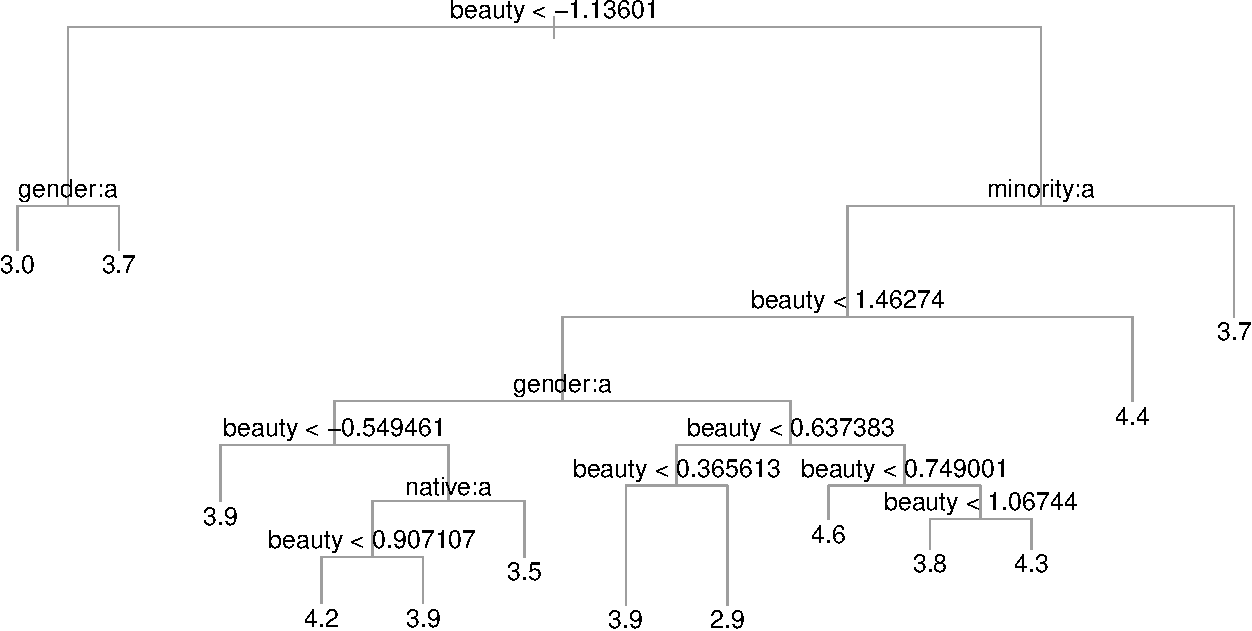
\includegraphics[scale=0.4]{figures/unnamed-chunk-3-1.pdf}              
 \end{figure}

\end{frame}

%----------------------------------------------------------------------%
\begin{frame}[fragile]
\frametitle{CART: Recap w. Example: Beauty in the classroom}
\framesubtitle{Trees: Constructing the partition}


\begin{itemize}
 \item How to choose the partition?
 \item Start with the trivial partition with one element
 \item  Greedy algorithm (CART): Iteratively split an element of the partition, such that the in-sample prediction improves as much as possible.
 \item That is: Given $(R_1\dots,R_M)$
 \begin{itemize}
  \item For each $R_m$ $m=1,\dots,M$ and
  \item For each $X_j$ $j=1,\dots,p$
  \item find the $s_{j,m}$ that minimizes the mean squared error, if we split $R_m$ along variable $X_j$ at $s_{j,m}$
  \item then pick the $(m,j)$ that minimizes the MSE and construct a new partition with $M+1$ elements
  \item Iterate
 \end{itemize}
 
\end{itemize}
\end{frame}

%----------------------------------------------------------------------%
\begin{frame}[fragile]
\frametitle{CART: Recap w. Example: Beauty in the classroom}
\framesubtitle{Trees: Tuning and pruning}

\begin{itemize}
\item Key tuning parameter: Total number of splits M.
\item We can optimize this via cross-validation.
\item CART can furthermore be improved using “pruning.”
\item Idea:
\begin{itemize}
\item Fit a flexible tree (with large M) using CART.
\item Then iteratively remove (collapse) nodes.
\item To minimize the sum of squared errors,
\item plus a penalty for the number of elements in the partition.
\end{itemize}

\item This improves upon greedy search. It yields smaller trees for the same mean squared error.
\end{itemize}

\end{frame}

%----------------------------------------------------------------------%
\begin{frame}[fragile]
\frametitle{CART: Recap w. Example: Beauty in the classroom}
\framesubtitle{Trees}

\begin{scriptsize}
\begin{Shaded}
\begin{Highlighting}[]
\CommentTok{\#\# Use cross{-}validation to prune the tree}
\NormalTok{cvpst \textless{}{-}}\StringTok{ }\KeywordTok{cv.tree}\NormalTok{(pstree, }\DataTypeTok{K=}\DecValTok{10}\NormalTok{)}
\KeywordTok{plot}\NormalTok{(cvpst}\OperatorTok{$}\NormalTok{size, cvpst}\OperatorTok{$}\NormalTok{dev, }\DataTypeTok{xlab=}\StringTok{"size"}\NormalTok{, }\DataTypeTok{ylab=}\StringTok{"oos deviance"}\NormalTok{, }\DataTypeTok{pch=}\DecValTok{21}\NormalTok{, }\DataTypeTok{bg=}\StringTok{"lightblue"}\NormalTok{, }\DataTypeTok{bty=}\StringTok{"n"}\NormalTok{)}
\end{Highlighting}
\end{Shaded}
\end{scriptsize}

\begin{figure}[H] \centering
            \captionsetup{justification=centering}
              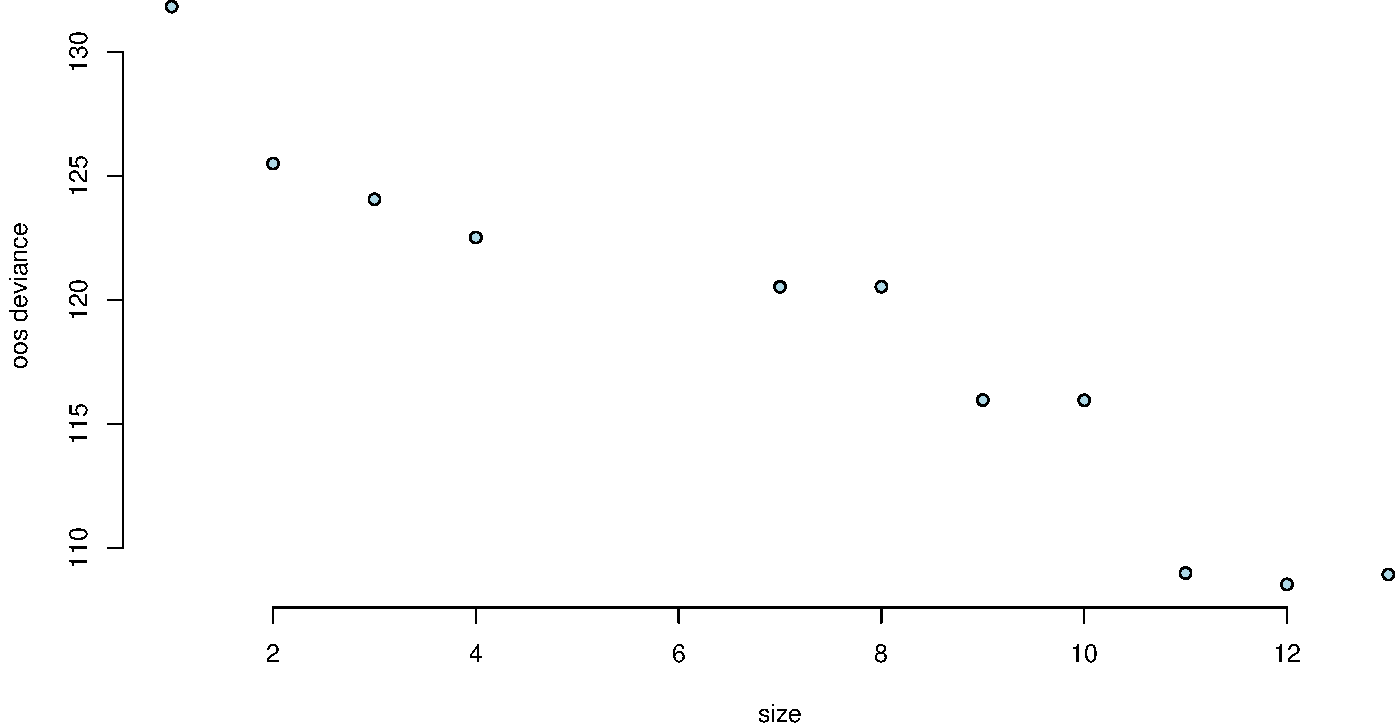
\includegraphics[scale=0.4]{figures/unnamed-chunk-4-1.pdf}              
 \end{figure}

\end{frame}

%----------------------------------------------------------------------%
\begin{frame}[fragile]
\frametitle{CART: Recap w. Example: Beauty in the classroom}
\framesubtitle{Trees}

\begin{scriptsize}
\begin{Shaded}
\begin{Highlighting}[]
\NormalTok{pstcut \textless{}{-}}\StringTok{ }\KeywordTok{prune.tree}\NormalTok{(pstree, }\DataTypeTok{best=}\DecValTok{12}\NormalTok{)}
\KeywordTok{plot}\NormalTok{(pstcut, }\DataTypeTok{col=}\DecValTok{8}\NormalTok{)}
\KeywordTok{text}\NormalTok{(pstcut)}
\end{Highlighting}
\end{Shaded}

\end{scriptsize}
\begin{figure}[H] \centering
            \captionsetup{justification=centering}
              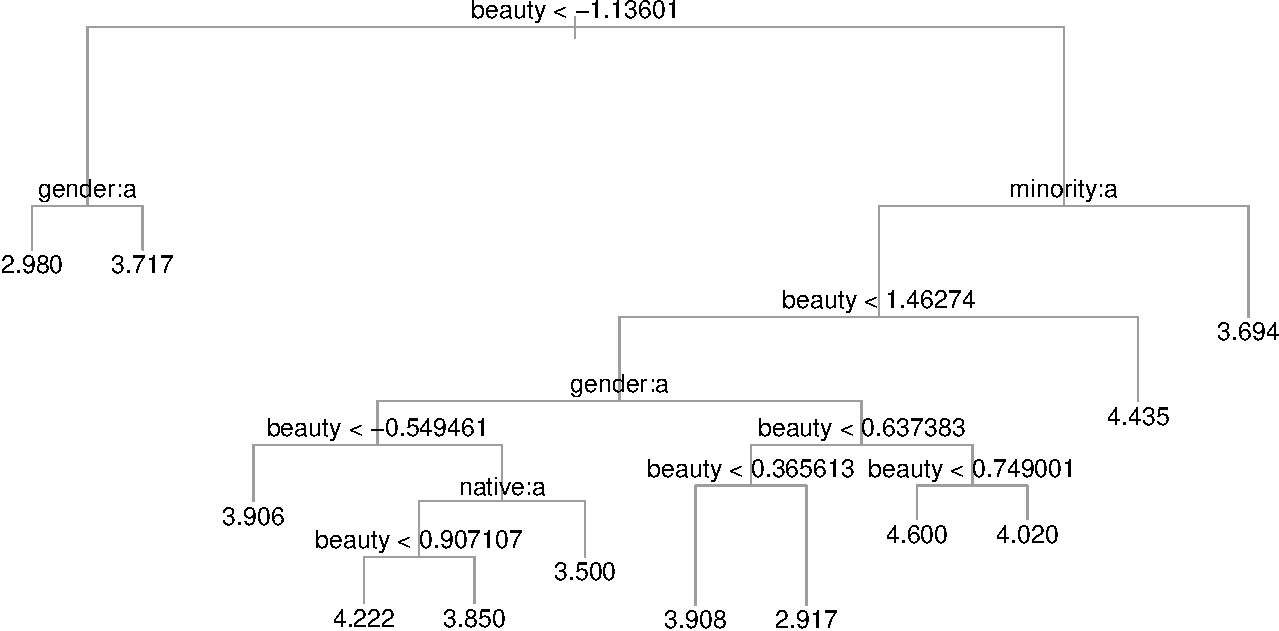
\includegraphics[scale=0.4]{figures/unnamed-chunk-6-1.pdf}              
 \end{figure}


\end{frame}

%----------------------------------------------------------------------%
\begin{frame}[fragile]
\frametitle{CARTs}

\begin{itemize}
  \item Smart way to represent nonlinearities. Most relevant variables on top.
  \medskip
  \item Very easy to communicate.
  \medskip
  \item  Reproduces human decision-making process.
  \medskip
  \item Trees are intuitive and do OK, but
  \begin{itemize}
    \item They are not very good at prediction 
  \item If the structure is linear, CART does not work well.
  \item  Not very robust
  \end{itemize}
  
\end{itemize}


\end{frame}
%----------------------------------------------------------------------%
\section{Causal Trees}
%----------------------------------------------------------------------%
%----------------------------------------------------------------------%

\begin{frame}[fragile]
\frametitle{}


\centering
{\huge \textcolor{andesred}{Causal Trees}}



\end{frame}
%----------------------------------------------------------------------%
%----------------------------------------------------------------------%
\subsection{Causality Review: ATE, CATE, HTE}
%----------------------------------------------------------------------%
\begin{frame}[fragile]
\frametitle{Treatment Effects Review}

\begin{itemize}
\item We observe a sequence of triples $\{(W_i, Y_i, X_i)\}_{i}^{N}$, where
\medskip

\begin{itemize}

\item \(W_{i} \in \{0, 1\}\): is a binary variable indicating whether the individual was treated (\(1\)) or not (\(0\))
\medskip
\item \(Y_{i}^{obs} \in \mathbb{R}\): a real variable indicating the observed outcome for that individual
\medskip
\item \(X_{i}\): is a \(p\)-dimensional vector of observable pre-treatment characteristics
\end{itemize}
\medskip
 \item Moreover, in the Neyman-Rubin potential-outcomes framework, we will denote by 
 \medskip
 \begin{itemize}
\item \(Y_{i}(1)\): the outcome unit \(i\) would attain if they received the  treatment
\medskip
\item \(Y_{i}(0)\): the outcome unit \(i\) would attain if they were part of the control group
\end{itemize}

\end{itemize}



\end{frame}
%----------------------------------------------------------------------%
\begin{frame}[fragile]
\frametitle{Treatment Effects Review}
 The individual treatment effect for subject $i$ can then be written as 

$$Y_i(1) - Y_i(0)$$

Unfortunately, in our data we can only observe one of these two potential outcomes. 

\begin{table}[H] 
\footnotesize \centering
 \begin{threeparttable} \captionsetup{justification=centering}   
\begin{tabular}{@{\extracolsep{5pt}}ccccc} \\[-1.8ex]
\hline \hline \\[-1.8ex]
Education & Treated & No Subsidy & Subsidy & Treatment effect \\
$(X_{i})$ & $W_i$ & $Y_{i}(0)$ & $Y_{i}(1)$ & $\tau_i=Y_{i}(1)-Y_{i}(0)$ \\
\midrule
$High$ & $1$ & ?          & $Y_{1}(1)$      & ?\\
$High$ & $0$ & $Y_{2}(0)$ & ?                & ? \\
$Low$  & $0$ & $Y_{3}(0)$ & ?              & ? \\
$Low$  & $1$ & ?          & $Y_{4}(1)$       & ? \\
  \\[-1.8ex]\hline        \hline \\[-1.8ex]        
  \end{tabular}         
\end{threeparttable}       
\end{table}       

Using the potential outcome notation above, the observed outcome can also be written as

\[Y_{i} = W_{i}Y_{i}(1) + (1-W_{i})Y_{i}(0)\]




\end{frame}
%----------------------------------------------------------------------%
\begin{frame}[fragile]
\frametitle{Average Treatment Effects Review}
\begin{itemize}
\item Computing the difference for each individual is impossible. 
\medskip
\item But we can get the Average Treatment Effect (ATE):

  \begin{align}
    \tau := E[Y_i(1) - Y_i(0)]
  \end{align}
  

  \item Heterogeneous Treatment Effects: Same treatment may affect different individuals differently
  \medskip
  \item Conditional Average Treatment Effect (CATE)
  \begin{align}
    \tau(x) := E[Y_i(1) - Y_i(0)|X_i=x]
  \end{align}
\end{itemize}


\end{frame}


%----------------------------------------------------------------------%
\begin{frame}[fragile]
\frametitle{Heterogeneous Treatment Effects Review}

\framesubtitle{Concerns}

\begin{itemize}
  \item Issues:
  
  \begin{itemize}
  \item Ad hoc searches for particularly responsive subgroups may mistake noise for a true treatment effect. 
  
  \item Concerns about ex-post “data-mining” or  p-hacking
    \begin{itemize}
      \item preregistered analysis plan can protect against claims of data mining  
      \item But may also prevent researchers from discovering unanticipated results and developing new hypotheses
    \end{itemize}
  \end{itemize}
\medskip
\item But how is researcher to predict all forms of heterogeneity in an environment with many covariates?
\medskip
\item Athey and Imbens to the rescue
\begin{itemize}
  \item Allow researcher to specify set of potential covariates
  \item Data-driven search for heterogeneity in causal effects with valid standard errors
\end{itemize}


\end{itemize}


\end{frame}



%----------------------------------------------------------------------%
\subsection{Empirical Example}
%----------------------------------------------------------------------%
\begin{frame}[fragile]
\frametitle{Causal Trees: Empirical Example (Green and Kern) }

\begin{itemize}
\item To illustrate how it works let me use this experiment from the General Social Survey (GSS)
\medskip
\item GSS conducts surveys regular surveys on Americans think feel about different issues
\medskip
 \item For decades, scholars studying Americans' support for social welfare spending have noted the special disdain that americans harbor for programs labeled “welfare” 
\medskip
 \item This phenomenon became the subject of sustained experimental inquiry in the mid-1980s, when the GSS included a question-wording experiment in its national survey of adults. 
 \medskip

\end{itemize}
\end{frame}
%----------------------------------------------------------------------%
\begin{frame}[fragile]
\frametitle{Causal Trees: Empirical Example }
\begin{itemize}
\item Respondents in each survey were randomly assigned to one of two questions about public spending.
 \medskip
\item {\it “too much” money is spent on assistance to the Poor (control) or Welfare (treatment)}
\medskip
\item Various explanations put forward: stereotypes  associated  with  welfare  recipients  and  poor  people, particularly racial stereotypes,  and  to  political  orientations  such  as  individualism  and  conservatism  .  
\item Some authors consider the  interaction  between  the  treatment  and  attributions,  e.g.
\begin{itemize}
 \item Federico  (2004)  examines  a  complicated  three-way  interaction  between  the  treatment,  education,  and  racial  perceptions.  
 \item Jacoby  (2000)  suggests  that  party  and  ideology  may make some respondents especially receptive to the more specific program (should strong and weak Democrats be treated as separate subgroups or should they be combined?)
\end{itemize}
\end{itemize}
\end{frame}
%----------------------------------------------------------------------%
\begin{frame}[fragile]
\frametitle{Causal Trees}

\begin{scriptsize}
\begin{Shaded}
\begin{Highlighting}[]
\CommentTok{\#load packages}
\KeywordTok{library}\NormalTok{(fBasics)     }\CommentTok{\# Summary statistics }
\KeywordTok{library}\NormalTok{(rpart)       }\CommentTok{\# Classification and regression trees}
\KeywordTok{library}\NormalTok{(rpart.plot)  }\CommentTok{\# Plotting trees}
\KeywordTok{library}\NormalTok{(treeClust)   }\CommentTok{\# Predicting leaf position for causal trees }
\KeywordTok{library}\NormalTok{(car)         }\CommentTok{\# linear hypothesis testing for causal tree}
\KeywordTok{library}\NormalTok{(kableExtra)  }\CommentTok{\# Tables}
\KeywordTok{library}\NormalTok{(causalTree) }\CommentTok{\# For causal trees (Athey and Imbens, 2016)  }
\KeywordTok{library}\NormalTok{(dplyr)} \CommentTok{\# For data wrangling }
\CommentTok{\# Set seed for reproducibility}
\KeywordTok{set.seed}\NormalTok{(}\DecValTok{201911}\NormalTok{) }
\CommentTok{\# Load Data}
\NormalTok{df\textless{}{-}}\KeywordTok{readRDS}\NormalTok{(}\StringTok{"welfare.rds"}\NormalTok{)}
\KeywordTok{str}\NormalTok{(df)}
\end{Highlighting}
\end{Shaded}
\end{scriptsize}
\begin{tiny}
\begin{verbatim}
'data.frame':   13198 obs. of  34 variables:
 $ ID      : int  1 2 3 4 5 6 7 8 9 10 ...
 $ Y       : num  0 0 1 1 1 0 0 0 1 0 ...
 $ W       : num  1 1 1 0 0 1 1 0 0 1 ...
 $ hrs1    : num  40 35 30 40 35 38 27 40 32 50 ...
 $ partyid : num  4 1 2 2 1 2 0 1 3 3 ...
 $ income  : num  12 12 12 12 11 12 12 11 12 12 ...
 ...
 
\end{verbatim}
\end{tiny}

\end{frame}
%----------------------------------------------------------------------%
\begin{frame}[fragile]
\frametitle{Causal Trees}
\framesubtitle{ATE}
 
\begin{tiny}
\begin{Shaded}
\begin{Highlighting}[]
\NormalTok{difference\_in\_means \textless{}{-}}\StringTok{ }\ControlFlowTok{function}\NormalTok{(dataset) \{}
\NormalTok{  treated\_idx \textless{}{-}}\StringTok{ }\KeywordTok{which}\NormalTok{(dataset}\OperatorTok{$}\NormalTok{W }\OperatorTok{==}\StringTok{ }\DecValTok{1}\NormalTok{)}
\NormalTok{  control\_idx \textless{}{-}}\StringTok{ }\KeywordTok{which}\NormalTok{(dataset}\OperatorTok{$}\NormalTok{W }\OperatorTok{==}\StringTok{ }\DecValTok{0}\NormalTok{)}
  
  \CommentTok{\# Filter treatment / control observations, pulls outcome variable as a vector}
\NormalTok{  y1 \textless{}{-}}\StringTok{ }\NormalTok{dataset[treated\_idx, }\StringTok{"Y"}\NormalTok{] }\CommentTok{\# Outcome in treatment grp}
\NormalTok{  y0 \textless{}{-}}\StringTok{ }\NormalTok{dataset[control\_idx, }\StringTok{"Y"}\NormalTok{] }\CommentTok{\# Outcome in control group}
  
\NormalTok{  n1 \textless{}{-}}\StringTok{ }\KeywordTok{sum}\NormalTok{(df[,}\StringTok{"W"}\NormalTok{])     }\CommentTok{\# Number of obs in treatment}
\NormalTok{  n0 \textless{}{-}}\StringTok{ }\KeywordTok{sum}\NormalTok{(}\DecValTok{1} \OperatorTok{{-}}\StringTok{ }\NormalTok{df[,}\StringTok{"W"}\NormalTok{]) }\CommentTok{\# Number of obs in control}
  
  \CommentTok{\# Difference in means is ATE}
\NormalTok{  tauhat \textless{}{-}}\StringTok{ }\KeywordTok{mean}\NormalTok{(y1) }\OperatorTok{{-}}\StringTok{ }\KeywordTok{mean}\NormalTok{(y0)}
  
  \CommentTok{\# 95\% Confidence intervals}
\NormalTok{  se\_hat \textless{}{-}}\StringTok{ }\KeywordTok{sqrt}\NormalTok{( }\KeywordTok{var}\NormalTok{(y0)}\OperatorTok{/}\NormalTok{(n0}\DecValTok{{-}1}\NormalTok{) }\OperatorTok{+}\StringTok{ }\KeywordTok{var}\NormalTok{(y1)}\OperatorTok{/}\NormalTok{(n1}\DecValTok{{-}1}\NormalTok{) )}
\NormalTok{  lower\_ci \textless{}{-}}\StringTok{ }\NormalTok{tauhat }\OperatorTok{{-}}\StringTok{ }\FloatTok{1.96} \OperatorTok{*}\StringTok{ }\NormalTok{se\_hat}
\NormalTok{  upper\_ci \textless{}{-}}\StringTok{ }\NormalTok{tauhat }\OperatorTok{+}\StringTok{ }\FloatTok{1.96} \OperatorTok{*}\StringTok{ }\NormalTok{se\_hat}
  
  \KeywordTok{return}\NormalTok{(}\KeywordTok{c}\NormalTok{(}\DataTypeTok{ATE =}\NormalTok{ tauhat, }\DataTypeTok{lower\_ci =}\NormalTok{ lower\_ci, }\DataTypeTok{upper\_ci =}\NormalTok{ upper\_ci))}
\NormalTok{\}}

\NormalTok{tauhat\_rct \textless{}{-}}\StringTok{ }\KeywordTok{difference\_in\_means}\NormalTok{(df)}
\NormalTok{tauhat\_rct}
\end{Highlighting}
\end{Shaded}
\end{tiny}

\begin{verbatim}
       ATE   lower_ci   upper_ci 
-0.3697802 -0.3841123 -0.3554481 
\end{verbatim}

\end{frame}
%----------------------------------------------------------------------%
\begin{frame}[fragile]
\frametitle{Causal Trees}
\framesubtitle{ATE}
\begin{scriptsize}
\begin{Shaded}
\begin{Highlighting}[]
\NormalTok{outcome\_variable\_name \textless{}{-}}\StringTok{ "Y"}
\NormalTok{treatment\_variable\_name \textless{}\textless{}{-}}\StringTok{ "W"}
\NormalTok{covariate\_names \textless{}\textless{}{-}}\StringTok{ }\KeywordTok{c}\NormalTok{(}\StringTok{"hrs1"}\NormalTok{, }\StringTok{"partyid"}\NormalTok{, }\StringTok{"income"}\NormalTok{, }\StringTok{"rincome"}\NormalTok{, }
                      \StringTok{"wrkstat"}\NormalTok{, }\StringTok{"wrkslf"}\NormalTok{,}\StringTok{"age"}\NormalTok{, }\StringTok{"polviews"}\NormalTok{,}
                      \StringTok{"educ"}\NormalTok{, }\StringTok{"earnrs"}\NormalTok{, }\StringTok{"race"}\NormalTok{,}\StringTok{"wrkslf"}\NormalTok{,}
                      \StringTok{"marital"}\NormalTok{,}\StringTok{"sibs"}\NormalTok{,}\StringTok{"childs"}\NormalTok{, }\StringTok{"occ80"}\NormalTok{,  }
                      \StringTok{"prestg80"}\NormalTok{, }\StringTok{"indus80"}\NormalTok{,}\StringTok{"res16"}\NormalTok{,}\StringTok{"reg16"}\NormalTok{,}
                      \StringTok{"mobile16"}\NormalTok{, }\StringTok{"family16"}\NormalTok{, }\StringTok{"parborn"}\NormalTok{,}
                      \StringTok{"maeduc"}\NormalTok{,}\StringTok{"degree"}\NormalTok{,}\StringTok{"sex"}\NormalTok{,}\StringTok{"race"}\NormalTok{,}
                      \StringTok{"born"}\NormalTok{,}\StringTok{"hompop"}\NormalTok{,}\StringTok{"babies"}\NormalTok{,}
                      \StringTok{"preteen"}\NormalTok{,}\StringTok{"teens"}\NormalTok{,}\StringTok{"adults"}\NormalTok{)}

\NormalTok{fmla \textless{}{-}}\StringTok{ }\KeywordTok{paste}\NormalTok{(}\StringTok{"Y \textasciitilde{} W +"}\NormalTok{,}\KeywordTok{paste}\NormalTok{(covariate\_names, }\DataTypeTok{collapse =} \StringTok{" + "}\NormalTok{))}
\KeywordTok{print}\NormalTok{( fmla)}
\end{Highlighting}
\end{Shaded}
\end{scriptsize}

\begin{tiny}
\begin{verbatim}
[1] "Y ~ W + hrs1 + partyid + income + rincome + wrkstat + wrkslf + age 
+ polviews + educ + earnrs + race + wrkslf + marital + sibs + childs 
+ occ80 + prestg80 + indus80 + res16 + reg16 + mobile16 + family16 
+ parborn + maeduc + degree + sex + race + born + hompop + babies + preteen + teens + adults"
\end{verbatim}
\end{tiny}

\end{frame}
%----------------------------------------------------------------------%
\begin{frame}[fragile]
\frametitle{Causal Trees}
\framesubtitle{ATE}
\begin{scriptsize}


\begin{Shaded}
\begin{Highlighting}[]
\NormalTok{reg\_simple\textless{}{-}}\KeywordTok{lm}\NormalTok{(Y}\OperatorTok{\textasciitilde{}}\NormalTok{W,}\DataTypeTok{data=}\NormalTok{df)}
\NormalTok{reg\_controls\textless{}{-}}\KeywordTok{lm}\NormalTok{(fmla,}\DataTypeTok{data=}\NormalTok{df)}
\NormalTok{stargazer}\OperatorTok{::}\KeywordTok{stargazer}\NormalTok{(reg\_simple,reg\_controls,}\DataTypeTok{type=}\StringTok{"latex"}\NormalTok{)}
\end{Highlighting}
\end{Shaded}
\end{scriptsize}


\begin{table}[!htbp] \centering 
  \caption{} 
  \label{} 
  \scriptsize
\begin{tabular}{@{\extracolsep{5pt}}lcc} 
\\[-1.8ex]\hline 
\hline \\[-1.8ex] 
 & \multicolumn{2}{c}{\textit{Dependent variable:}} \\ 
\cline{2-3} 
\\[-1.8ex] & \multicolumn{2}{c}{Y} \\ 
\\[-1.8ex] & (1) & (2)\\ 
\hline \\[-1.8ex] 
 W & $-$0.370$^{***}$ & $-$0.368$^{***}$ \\ 
  & (0.007) & (0.007) \\ 
  & & \\ 
 
 Constant & 0.481$^{***}$ & 0.223$^{***}$ \\ 
  & (0.005) & (0.069) \\ 
  & & \\ 
\hline \\[-1.8ex] 
Controls & No & Yes \\ 
Observations & 13,198 & 13,198 \\ 
R$^{2}$ & 0.166 & 0.215 \\ 
\hline 
\hline \\[-1.8ex] 
\textit{Note:}  & \multicolumn{2}{r}{$^{*}$p$<$0.1; $^{**}$p$<$0.05; $^{***}$p$<$0.01} \\ 
\end{tabular} 
\end{table} 

\end{frame}

%----------------------------------------------------------------------%
\begin{frame}[fragile]
\frametitle{Causal Trees}
\framesubtitle{HTE}

\begin{itemize}
 \item We need to proceed in steps
 \item Step 1: Split the dataset. Why? $\rightarrow$ Athey and Imbens innovation
 \begin{itemize}
  \item In order to ensure valid estimates of the treatment effect within each subgroup, Athey and Imbens propose a sample-splitting approach that they refer to as honesty: 
  \item a method is honest if it uses one subset of the data to estimate the model parameters, and a different subset to produce estimates given these estimated parameters. 
  \item In the context of causal trees, honesty implies that the asymptotic properties of treatment effect estimates within leaves are the same as if the tree partition had been exogenously given, and it is one of the assumptions required to produce unbiased and asymptotically normal estimates of the treatment effect.
 
 \end{itemize}
\end{itemize}

\end{frame}

%----------------------------------------------------------------------%
\begin{frame}[fragile]
\frametitle{Causal Trees}
\framesubtitle{HTE}

\begin{itemize}
\item Divide the data 40\%-40\%-20\% for honest estimation and validation.
\end{itemize}

\begin{scriptsize}


\begin{Shaded}
\begin{Highlighting}[]
\NormalTok{train\_fraction \textless{}{-}}\StringTok{ }\FloatTok{0.80}  \CommentTok{\# Use train\_fraction \% of the dataset to train our models}

\NormalTok{df\_train \textless{}{-}}\StringTok{ }\KeywordTok{sample\_frac}\NormalTok{(df, }\DataTypeTok{replace=}\NormalTok{F, }\DataTypeTok{size=}\NormalTok{train\_fraction)}
\NormalTok{df\_test \textless{}{-}}\StringTok{ }\KeywordTok{anti\_join}\NormalTok{(df,df\_train, }\DataTypeTok{by =} \StringTok{"ID"}\NormalTok{)}\CommentTok{\#need to check on larger datasets}


\NormalTok{split\_size \textless{}{-}}\StringTok{ }\KeywordTok{floor}\NormalTok{(}\KeywordTok{nrow}\NormalTok{(df\_train) }\OperatorTok{*}\StringTok{ }\FloatTok{0.5}\NormalTok{)}
\NormalTok{df\_split \textless{}{-}}\StringTok{ }\KeywordTok{sample\_n}\NormalTok{(df\_train, }\DataTypeTok{replace=}\OtherTok{FALSE}\NormalTok{, }\DataTypeTok{size=}\NormalTok{split\_size)}

\CommentTok{\# Make the splits}
\NormalTok{df\_est \textless{}{-}}\StringTok{ }\KeywordTok{anti\_join}\NormalTok{(df\_train,df\_split, }\DataTypeTok{by =}\StringTok{"ID"}\NormalTok{)}
\end{Highlighting}
\end{Shaded}
\end{scriptsize}

\end{frame}

%----------------------------------------------------------------------%
\begin{frame}[fragile]
\frametitle{Causal Trees}

\begin{itemize}
  \item Step 2: Fit the tree
\end{itemize}

\begin{scriptsize}
\begin{Shaded}
\begin{Highlighting}[]
\NormalTok{fmla\_ct \textless{}{-}}\StringTok{ }\KeywordTok{paste}\NormalTok{(}\StringTok{"factor(Y) \textasciitilde{}"}\NormalTok{, }\KeywordTok{paste}\NormalTok{(covariate\_names, }\DataTypeTok{collapse =} \StringTok{" + "}\NormalTok{))}

\NormalTok{ct\_unpruned \textless{}{-}}\StringTok{ }\KeywordTok{honest.causalTree}\NormalTok{(}
  \DataTypeTok{formula =}\NormalTok{ fmla\_ct,            }\CommentTok{\# Define the model}
  \DataTypeTok{data =}\NormalTok{ df\_split,              }\CommentTok{\# Subset used to create tree structure}
  \DataTypeTok{est\_data =}\NormalTok{ df\_est,            }\CommentTok{\# Which data set to use to estimate effects}

  \DataTypeTok{treatment =}\NormalTok{ df\_split}\OperatorTok{$}\NormalTok{W,       }\CommentTok{\# Splitting sample treatment variable}
  \DataTypeTok{est\_treatment =}\NormalTok{ df\_est}\OperatorTok{$}\NormalTok{W,     }\CommentTok{\# Estimation sample treatment variable}

  \DataTypeTok{split.Rule =} \StringTok{"CT"}\NormalTok{,            }\CommentTok{\# Define the splitting option}
  \DataTypeTok{cv.option =} \StringTok{"TOT"}\NormalTok{,            }\CommentTok{\# Cross validation options}
  \DataTypeTok{cp =} \DecValTok{0}\NormalTok{,                       }\CommentTok{\# Complexity parameter}

  \DataTypeTok{split.Honest =} \OtherTok{TRUE}\NormalTok{,          }\CommentTok{\# Use honesty when splitting}
  \DataTypeTok{cv.Honest =} \OtherTok{TRUE}\NormalTok{,             }\CommentTok{\# Use honesty when performing cross{-}validation}

  \DataTypeTok{minsize =} \DecValTok{25}\NormalTok{,                 }\CommentTok{\# Min. number of treatment and control cases in each leaf}
  \DataTypeTok{HonestSampleSize =} \KeywordTok{nrow}\NormalTok{(df\_est)) }\CommentTok{\# Num obs used in estimation after building the tree}
\end{Highlighting}
\end{Shaded}
\end{scriptsize}


\end{frame}
%----------------------------------------------------------------------%
\begin{frame}[fragile]
\frametitle{Causal Trees}

\begin{itemize}
\item Step 3: Crossvalidate
\end{itemize}

\begin{scriptsize}
\begin{Shaded}
\begin{Highlighting}[]
\CommentTok{\# Table of cross{-}validated values by tuning parameter.}
\NormalTok{ct\_cptable \textless{}{-}}\StringTok{ }\KeywordTok{as.data.frame}\NormalTok{(ct\_unpruned}\OperatorTok{$}\NormalTok{cptable)}
\CommentTok{\# Obtain optimal complexity parameter to prune tree.}
\NormalTok{selected\_cp \textless{}{-}}\StringTok{ }\KeywordTok{which.min}\NormalTok{(ct\_cptable}\OperatorTok{$}\NormalTok{xerror)}
\NormalTok{optim\_cp\_ct \textless{}{-}}\StringTok{ }\NormalTok{ct\_cptable[selected\_cp, }\StringTok{"CP"}\NormalTok{]}
\CommentTok{\# Prune the tree at optimal complexity parameter.}
\NormalTok{ct\_pruned \textless{}{-}}\StringTok{ }\KeywordTok{prune}\NormalTok{(}\DataTypeTok{tree =}\NormalTok{ ct\_unpruned, }\DataTypeTok{cp =}\NormalTok{ optim\_cp\_ct)}
\NormalTok{ct\_pruned}
\end{Highlighting}
\end{Shaded}
\end{scriptsize}

\begin{tiny}
\begin{verbatim}
n= 5279 

node), split, n, deviance, yval
      * denotes terminal node

 1) root 5279 912.78610 -0.3753160  
   2) partyid>=1.5 3530 654.60930 -0.3822570  
     4) polviews>=3.5 2826 532.11460 -0.3997024  
       8) reg16>=0.5 2658 500.98290 -0.4043439  
        16) hrs1>=44.5 1063 203.85490 -0.4271320  
          32) wrkslf< 1.5 182  35.70208 -0.4264330  
            64) indus80< 526 81  15.81056 -0.3757764 *
            65) indus80>=526 101  19.59552 -0.4610849 *
          33) wrkslf>=1.5 881 167.91090 -0.4283712 *
        17) hrs1< 44.5 1595 295.01770 -0.3896395 *
       9) reg16< 0.5 168  30.09444 -0.3315372 *
     5) polviews< 3.5 704 115.34030 -0.3167446 *
   3) partyid< 1.5 1749 245.33770 -0.3548876  
     6) maeduc< 14.5 1476 210.08960 -0.3843850 *
     7) maeduc>=14.5 273  31.06203 -0.2124060 *
\end{verbatim}

\end{tiny}

\end{frame}
%----------------------------------------------------------------------%
\begin{frame}[fragile]
\frametitle{Causal Trees}

\begin{itemize}
\item Step 4: Predict point estimates (on estimation sample)
\end{itemize}



\begin{Shaded}
\begin{Highlighting}[]
\NormalTok{tauhat\_ct\_est \textless{}{-}}\StringTok{ }\KeywordTok{predict}\NormalTok{(ct\_pruned, }\DataTypeTok{newdata =}\NormalTok{ df\_est)}
\KeywordTok{head}\NormalTok{(tauhat\_ct\_est)}
\end{Highlighting}
\end{Shaded}

\begin{verbatim}
         1          2          3          4          5          6 
-0.3843850 -0.4283712 -0.3843850 -0.3896395 -0.3896395 -0.3843850 
\end{verbatim}

\end{frame}
%----------------------------------------------------------------------%
\begin{frame}[fragile]
\frametitle{Causal Trees}

\begin{itemize}
\item Step 5: Compute standard errors
\item The \texttt{causalTree} package does not compute standard errors by default, but we can compute them using the following trick. 
\begin{itemize}
\item First, define $L_l$ to indicate assignment to leaf $l$
\item Second, consider the following linear model.
\begin{align}
  Y= \sum_l L_l \alpha_l + W L_l \beta_l
\end{align}
\item The interaction coefficients in this regression recover the average treatment effects in each leaf, since

\begin{align}
E[Y|W=1,L=1]-E[Y|W=0,L=1] = (\alpha_1+\beta_1)-\alpha_1=\beta_1
\end{align}

\item Therefore, the standard error around the coefficients is also the standard error around the treatment effects. 
\item We will also use these statistics to test hypothesis about leaf estimates.

\end{itemize}
\end{itemize}

\end{frame}
%----------------------------------------------------------------------%
\begin{frame}[fragile]
\frametitle{Causal Trees}



\begin{scriptsize}

\begin{Shaded}
\begin{Highlighting}[]
\CommentTok{\# Create a factor column \textquotesingle{}leaf\textquotesingle{} indicating leaf assignment}
\NormalTok{num\_leaves \textless{}{-}}\StringTok{ }\KeywordTok{length}\NormalTok{(}\KeywordTok{unique}\NormalTok{(tauhat\_ct\_est))  }\CommentTok{\#There are as many leaves as there are predictions}
\NormalTok{df\_est}\OperatorTok{$}\NormalTok{leaf \textless{}{-}}\StringTok{ }\KeywordTok{factor}\NormalTok{(tauhat\_ct\_est, }\DataTypeTok{labels =} \KeywordTok{seq}\NormalTok{(num\_leaves))}
\CommentTok{\# Run the regression}
\NormalTok{ols\_ct \textless{}{-}}\StringTok{ }\KeywordTok{lm}\NormalTok{(}\KeywordTok{as.formula}\NormalTok{(}\StringTok{"Y \textasciitilde{} 0 + leaf + W:leaf"}\NormalTok{), }\DataTypeTok{data=}\NormalTok{ df\_est) }
\NormalTok{ols\_ct\_summary \textless{}{-}}\StringTok{ }\KeywordTok{summary}\NormalTok{(ols\_ct)}
\end{Highlighting}
\end{Shaded}
\end{scriptsize}

\begin{table}
\scriptsize
\caption{\label{tab:unnamed-chunk-12}Average treatment effects per leaf}
\centering
\begin{tabular}[t]{l|r|r}
\hline
  & Estimate & Std. Error\\
\hline
leaf1:W & -0.4611 & 0.0817\\
\hline
leaf2:W & -0.4284 & 0.0276\\
\hline
leaf3:W & -0.3896 & 0.0205\\
\hline
leaf4:W & -0.3844 & 0.0214\\
\hline
leaf5:W & -0.3758 & 0.0920\\
\hline
leaf6:W & -0.3315 & 0.0633\\
\hline
leaf7:W & -0.3167 & 0.0309\\
\hline
leaf8:W & -0.2124 & 0.0497\\
\hline
\end{tabular}
\end{table}


\end{frame}
%----------------------------------------------------------------------%
\begin{frame}[fragile]
\frametitle{Causal Trees}
\begin{itemize}
  \item Step 6: Predict point estimates (on test set)
\end{itemize}

\begin{scriptsize}


\begin{Shaded}
\begin{Highlighting}[]
\NormalTok{tauhat\_ct\_test \textless{}{-}}\StringTok{ }\KeywordTok{predict}\NormalTok{(ct\_pruned, }\DataTypeTok{newdata =}\NormalTok{ df\_test)}


\KeywordTok{rpart.plot}\NormalTok{(}
  \DataTypeTok{x =}\NormalTok{ ct\_pruned,        }\CommentTok{\# Pruned tree}
  \DataTypeTok{type =} \DecValTok{3}\NormalTok{,             }\CommentTok{\# Draw separate split labels for the left and right directions}
  \DataTypeTok{fallen =} \OtherTok{TRUE}\NormalTok{,        }\CommentTok{\# Position the leaf nodes at the bottom of the graph}
  \DataTypeTok{leaf.round =} \DecValTok{1}\NormalTok{,       }\CommentTok{\# Rounding of the corners of the leaf node boxes}
  \DataTypeTok{extra =} \DecValTok{100}\NormalTok{,          }\CommentTok{\# Display the percentage of observations in the node}
  \DataTypeTok{branch =} \FloatTok{0.1}\NormalTok{,          }\CommentTok{\# Shape of the branch lines}
  \DataTypeTok{box.palette =} \StringTok{"RdBu"}\NormalTok{) }\CommentTok{\# Palette for coloring the node}
\end{Highlighting}
\end{Shaded}
\end{scriptsize}

\end{frame}
%----------------------------------------------------------------------%
\begin{frame}[fragile]
\frametitle{Causal Trees}

\begin{figure}[H] \centering
            \captionsetup{justification=centering}
            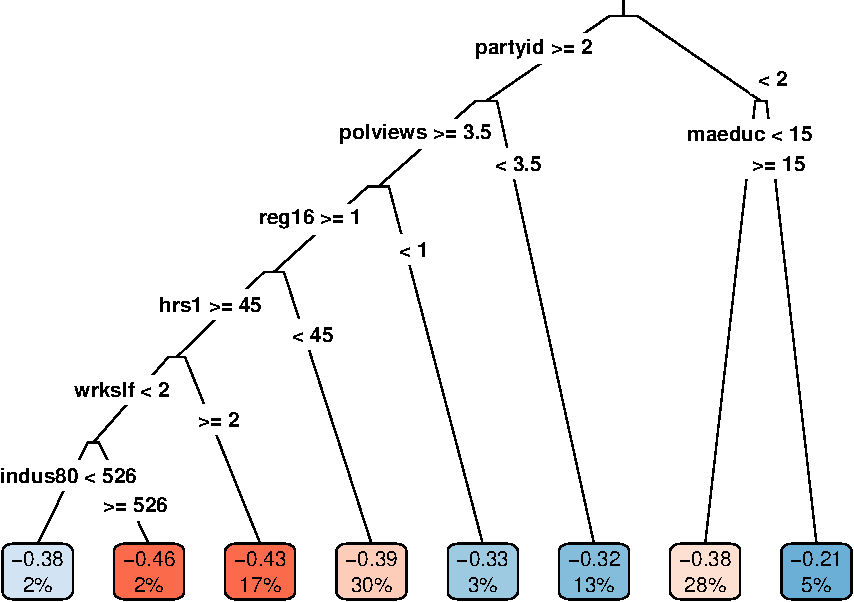
\includegraphics[scale=0.6]{figures/unnamed-chunk-14-1.pdf}
              
 \end{figure}



\end{frame}
%----------------------------------------------------------------------%
\begin{frame}[fragile]
\frametitle{Causal Trees}

\begin{scriptsize}


\begin{Shaded}
\begin{Highlighting}[]
\CommentTok{\# Null hypothesis: all leaf values are the same}
\NormalTok{hypothesis \textless{}{-}}\StringTok{ }\KeywordTok{paste0}\NormalTok{(}\StringTok{"leaf1:W = leaf"}\NormalTok{, }\KeywordTok{seq}\NormalTok{(}\DecValTok{2}\NormalTok{, num\_leaves), }\StringTok{":W"}\NormalTok{)}
\NormalTok{ftest \textless{}{-}}\StringTok{ }\KeywordTok{linearHypothesis}\NormalTok{(ols\_ct, hypothesis, }\DataTypeTok{test=}\StringTok{"F"}\NormalTok{)}

\KeywordTok{kable\_styling}\NormalTok{(}\KeywordTok{kable}\NormalTok{(}\KeywordTok{data.frame}\NormalTok{(ftest, }\DataTypeTok{check.names =} \OtherTok{FALSE}\NormalTok{, }\DataTypeTok{row.names =} \OtherTok{NULL}\NormalTok{)[}\DecValTok{2}\NormalTok{,],}
                    \StringTok{"latex"}\NormalTok{, }\DataTypeTok{digits =} \DecValTok{4}\NormalTok{,}
                    \DataTypeTok{caption=}\StringTok{"Testing null hypothesis: Average treatment effect is same across leaves"}\NormalTok{),}
              \DataTypeTok{bootstrap\_options=}\KeywordTok{c}\NormalTok{(}\StringTok{"striped"}\NormalTok{, }\StringTok{"hover"}\NormalTok{, }\StringTok{"condensed"}\NormalTok{, }\StringTok{"responsive"}\NormalTok{),}
              \DataTypeTok{full\_width=}\OtherTok{FALSE}\NormalTok{)}
\end{Highlighting}
\end{Shaded}
\end{scriptsize}

\begin{table}

\caption{\label{tab:unnamed-chunk-15}Testing null hypothesis: Average treatment effect is same across leaves}
\centering
\begin{tabular}[t]{l|r|r|r|r|r|r}
\hline
  & Res.Df & RSS & Df & Sum of Sq & F & Pr($>F$)\\
\hline
2 & 5263 & 884.921 & 7 & 3.4114 & 2.8984 & 0.005\\
\hline
\end{tabular}
\end{table}

\end{frame}


%----------------------------------------------------------------------%
\section{Causal Trees: Theory Details}
%----------------------------------------------------------------------%
\begin{frame}[fragile]
\frametitle{}


\centering
{\huge \textcolor{andesred}{Causal Trees: Theory Details}}



\end{frame}
%----------------------------------------------------------------------%

\begin{frame}[fragile]
\frametitle{}


\centering
{\huge \textcolor{andesred}{Causal Trees: Theory Details}}



\end{frame}

%----------------------------------------------------------------------%
\begin{frame}[fragile]
\frametitle{Causal Tree: Theory Details}



\begin{itemize}
  \item Work well in RCTs
  \medskip
  \item Issue: we do not observe the ground truth
  \medskip
  \item Honest estimation (Innovation):
    \begin{itemize}
      \item One sample to choose partition 
      \medskip
      \item One sample to estimate leaf effects
      \medskip
    \end{itemize}
  \item Why is the split critical?
  \medskip
  \item Fitting both on the training sample risks overfitting: Estimating many “heterogeneous effects” that are really just noise idiosyncratic to the sample.
  \medskip
  \item We want to search for true heterogeneity, not noise
\end{itemize}

\end{frame}


%----------------------------------------------------------------------%
\begin{frame}[fragile]
\frametitle{Heterogeneous Treatment Effects Assumptions}

\begin{itemize}
\item Before proceeding we need to make a couple of assumptions




\item Assumption 1: Unconfoundedness
\begin{align}
Y_i(1), Y_i(0) \perp W_i \ | \ X_i
\end{align}
\begin{itemize}
\item The \emph{unconfoundedness} assumption states that, once we condition on observable characteristics, the treatment assignment is independent to
how each person would respond to the treatment. 
\item i.e.,  the rule that determines whether or not a person is treated is determined completely by their observable characteristics. 
\item This allows, for example, for experiments where people from different genders get treated with different probabilities, 
\item {\bf rules out} experiments where people self-select into treatment due to some characteristic that is not observed in our data.

\end{itemize}


\end{itemize}




\end{frame}
%----------------------------------------------------------------------%
\begin{frame}[fragile]
\frametitle{Heterogeneous Treatment Effects}

\begin{itemize}
\item Assumption 2: Overlap
\medskip
\begin{align}
\forall \ x \in \text{supp}\ (X), \qquad 0 < P\ (W = 1 \ | \ X = x)  < 1
\end{align}

  \begin{itemize}
  \item The \emph{overlap} assumption states that at every point of the covariate space we can always find treated and control individuals.
  \medskip
  \item  i.e., in order to estimate the treatment effect for a person with particular  characteristics \(X_{i} = x\), we need to ensure that we are able to
  observe treated and untreated people with those same characteristics so that we can compare their outcomes. 
  \end{itemize}
\end{itemize}




\end{frame}
%----------------------------------------------------------------------%
\begin{frame}[fragile]
\frametitle{Trees}
\begin{itemize}
\item A simple tree

\begin{table}[]
\begin{tabular}{lll}
$MSE_0=\frac{1}{N}\sum(Y_i-\bar{Y})^2$ & \multicolumn{2}{l}{All observations} \\
\\
$MSE_1=\frac{1}{N}\sum(Y_i-\bar{Y}_{j:x_j\in l(x_i|\Pi)})^2$   & $X_i < c_1$      & $X_i \geq c_2$    
\end{tabular}
\end{table}
\bigskip
\item Partition $\Pi \in P$
  \begin{align}
  \left\{l_1=\{x_i : x_i< c_1\},l_2=\{x_i : x_i \geq c_2\} \right\}
  \end{align}
\item Prediction is 
  \begin{align}
  \hat{\mu}(x)=\bar{Y}_{j:x_j\in l(x_i|\Pi)}
  \end{align}

\end{itemize}
\end{frame}
%----------------------------------------------------------------------%
\begin{frame}[fragile]
\frametitle{The Honest Target: Athey and Imbens Innovation}

\begin{itemize}
\item Given a partition $\Pi$ define
\begin{align}
MSE_{\mu}(S^{te},S^{est},\Pi)=\frac{1}{\#(S^{te})}\sum_{i\in S^{te}}\left\{ \left(Y_{i}-\hat{\mu}(X_{i},S^{est},\Pi)\right)^{2}-Y_{i}^{2}\right\} 
\end{align}


\bigskip
\item The expected MSE is the expectation of $MSE_{\mu}(S^{te},S^{est},\Pi)$ over estimation and test samples (independent)

\begin{align}
EMSE_{\mu}(\Pi)=E_{S^{te},S^{est}}\left[MSE_{\mu}(S^{te},S^{est},\Pi)\right]
\end{align}


\end{itemize}

\end{frame}
%----------------------------------------------------------------------%
\begin{frame}[fragile]
\frametitle{The Honest Target: Athey and Imbens Innovation}


\begin{itemize}
\item The ultimate goal is to construct and assess an algorithm $\pi(.)$ that maximizes the honest criterion

\medskip
\begin{align}
max\,Q^{H}(\pi)=-E_{S^{te},S^{est},S^{tr}}\left[MSE_{\mu}(S^{te},S^{est},S^{tr},\pi(S^{tr})\right]
\end{align}


\item In CART the target is different (adaptive target)
\medskip
\begin{align}
max\,Q^{C}(\pi)=-E_{S^{te},S^{tr}}\left[MSE_{\mu}(S^{te},S^{tr},\pi(S^{tr})\right]
\end{align}


\end{itemize}
\end{frame}
%----------------------------------------------------------------------%
\begin{frame}[fragile]
\frametitle{The Honest Criterion}

\begin{align}
max\,Q^{H}(\pi)=-E_{S^{te},S^{est},S^{tr}}\left[MSE_{\mu}(S^{te},S^{est},S^{tr},\pi(S^{tr})\right]
\end{align}
\bigskip

$\,$ \\
\bigskip

$\,$\\
\bigskip

$\,$\\
\bigskip
\end{frame}
%----------------------------------------------------------------------%
\begin{frame}[fragile]
\frametitle{The Honest Criterion}

\begin{itemize}
  \item Understanding $EMSE_{\mu}(\Pi)$:
\end{itemize}
\begin{equation}
-EMSE_{\mu}(\Pi)=-E_{S^{te},S^{est}}\left[\left(Y_{i}-\hat{\mu}(X_{i},S^{est},\Pi)\right)^{2}-Y_{i}^{2}\right]
\end{equation}

\[
=-E_{S^{te},S^{est}}\left[\left(Y_{i}-\mu(X_{i},\Pi)+\mu(X_{i},\Pi)-\hat{\mu}(X_{i},S^{est},\Pi)\right)^{2}-Y_{i}^{2}\right]
\]

\[
=-E_{S^{te},S^{est}}\left[\left(Y_{i}-\mu(X_{i},\Pi)\right)^{2}-Y_{i}^{2}\right]
\]

\[
-E_{S^{te},S^{est}}\left[\left(\mu(X_{i},\Pi)-\hat{\mu}(X_{i},S^{est},\Pi)\right)^{2}\right]
\]

\[
-E_{S^{te},S^{est}}\left[2\left(Y_{i}-\mu(X_{i},\Pi)\right)\left(\mu(X_{i},\Pi)-\hat{\mu}(X_{i},S^{est},\Pi)\right)^{2}\right]
\]

\end{frame}
%----------------------------------------------------------------------%
\begin{frame}[fragile]
\frametitle{Heterogeneous Treatment Effects}




\[
=-E_{(Y_{i},X_{i}),S^{est}}\left[\left(Y_{i}-\mu(X_{i},\Pi)\right)^{2}-Y_{i}^{2}\right]-E_{X_{i},S^{est}}\left[\left(\mu(X_{i},\Pi)-\hat{\mu}(X_{i},S^{est},\Pi)\right)^{2}\right]
\]

\[
=-E_{(Y_{i},X_{i}),S^{est}}\left[Y_{i}^{2}-2Y_{i}\mu(X_{i},\Pi)+\mu^{2}(X_{i},\Pi)-Y_{i}^{2}\right]-E_{X_{i},S^{est}}\left[\left(\mu(X_{i},\Pi)-\hat{\mu}(X_{i},S^{est},\Pi)\right)^{2}\right]
\]

\[
=-E_{(Y_{i},X_{i}),S^{est}}\left[-2Y_{i}\mu(X_{i},\Pi)+\mu^{2}(X_{i},\Pi)\right]-E_{X_{i},S^{est}}\left[\left(\mu(X_{i},\Pi)-\hat{\mu}(X_{i},S^{est},\Pi)\right)^{2}\right]
\]



Note $E_{(Y_{i},X_{i}),S^{est}}(Y_{i})=E_{X_{i},s^{est}}\mu(X_{i},\Pi)$

\[
=-E_{(Y_{i},X_{i}),S^{est}}\left[\mu^{2}(X_{i},\Pi)\right]-E_{X_{i},S^{est}}\left[V(\hat{\mu}(X_{i},S^{est},\Pi))\right]
\]



\end{frame}
%----------------------------------------------------------------------%
\begin{frame}[fragile]
\frametitle{The Honest Criterion}

\begin{itemize}
 \item How to estimate this quantities?
 \item First $E_{X_{i},S^{est}}\left[V(\hat{\mu}(X_{i},S^{est},\Pi))\right]$
\end{itemize}

\[
V(\hat{\mu}(X_{i},S^{est},\Pi))=\frac{S_{S^{tr}}^{2}\left(l\left(x|\Pi\right)\right)}{N^{est}\left(l\left(x|\Pi\right)\right)}
\]

\[
\hat{E}_{X_{i},S^{est}}\left[V(\hat{\mu}(X_{i},S^{est},\Pi))|i\in S^{te}\right]=\sum_{l}p_{l}\frac{S_{S^{tr}}^{2}\left(l\right)}{N^{est}\left(l\right)}
\]

\[
=\sum_{l}\frac{1}{\#(l)}\frac{S_{S^{tr}}^{2}\left(l\right)}{N^{est}\left(l\right)}
\]

\[
=\frac{1}{N^{est}}\sum_{l\in\Pi}S_{S^{tr}}^{2}\left(l\right)
\]

\end{frame}
%----------------------------------------------------------------------%
\begin{frame}[fragile]
\frametitle{The Honest Criterion}


\begin{itemize}
  \item Next $E_{(Y_{i},X_{i}),S^{est}}\left[\mu^{2}(X_{i},\Pi)\right]$
  \item Note $V(\hat{\mu}|x,\Pi)=E(\hat{\mu}^{2}|x,\Pi)-\left[E(\hat{\mu}|x,\Pi)\right]^{2}$
\end{itemize}




\[
\frac{S_{S^{tr}}^{2}\left(l\left(x|\Pi\right)\right)}{N^{tr}\left(l\left(x|\Pi\right)\right)}\approx\hat{\mu}^{2}(x|S^{tr},\Pi)-\mu^{2}(x|\Pi)
\]

\[
\mu^{2}(x|\Pi)\approx\hat{\mu}^{2}(x|S^{tr},\Pi)-\frac{S_{S^{tr}}^{2}\left(l\left(x|\Pi\right)\right)}{N^{tr}\left(l\left(x|\Pi\right)\right)}
\]

\[
\hat{E}_{X_{i}}\left(\mu^{2}(X_{i}|\Pi\right)\approx\frac{1}{N^{tr}}\sum_{i\in S^{tr}}\hat{\mu}^{2}(x|S^{tr},\Pi)-\sum_{l}\frac{1}{\#l}\frac{S_{S^{tr}}^{2}\left(l\right)}{N^{tr}/\#l}
\]

\end{frame}
%----------------------------------------------------------------------%
\begin{frame}[fragile]
\frametitle{The Honest Criterion}


\begin{itemize}
  \item Finally
\end{itemize}

\[
-EMSE_{\mu}(\Pi)=\frac{1}{N^{tr}}\sum_{i\in S^{tr}}\hat{\mu}^{2}(x|S^{tr},\Pi)-\sum_{l}\frac{1}{N^{tr}}S_{S^{tr}}^{2}\left(l\right)-\frac{1}{N^{est}}\sum_{l\in\Pi}S_{S^{tr}}^{2}\left(l\right)
\]

\[
=\frac{1}{N^{tr}}\sum_{i\in S^{tr}}\hat{\mu}^{2}(x|S^{tr},\Pi)-\left(\frac{1}{N^{tr}}+\frac{1}{N^{est}}\right)\sum_{l\in\Pi}S_{S^{tr}}^{2}\left(l\right)
\]

\end{frame}
%----------------------------------------------------------------------%
\subsection{Honest Inference for Treatment Effects}
%----------------------------------------------------------------------%
\begin{frame}[fragile]
\frametitle{Honest Inference for Treatment Effects}

\begin{itemize}
\item Given a tree $\Pi$, define for all x and both treatment levels w the population average outcome



\[
\mu(w,x|\Pi)=E\left[Y_{i}(w)|X_{i}\in l(x|\Pi)\right]
\]

\item The Average Treatment Effect

\[
\tau(x|\Pi)=E\left[Y_{i}(1)-Y_{i}(0)|X_{i}\in l(x|\Pi)\right]
\]

\[
=\mu(1,x|\Pi)-\mu(0,x|\Pi)
\]
\end{itemize}
\end{frame}
%----------------------------------------------------------------------%
\begin{frame}[fragile]
\frametitle{Honest Inference for Treatment Effects}

\begin{itemize}
  \item The estimated counterparts are




\begin{align}
\hat{\mu}(w,x|S,\Pi)=\frac{1}{\#\left(\left\{ i\in S_{w}:X_{i}\in l(x|\Pi)\right\} \right)}\sum_{i\in S_{w}:X_{i}\in l(x|\Pi)}Y_{i}^{obs}
\end{align}

\begin{align}
\hat{\tau}(X,S,\Pi) = \hat{\mu}(1,x|S,\Pi) - \hat{\mu}(0,x|S,\Pi)
\end{align}

\item Define the MSE for treatment effects as

\[
MSE_{\tau}(S^{te},S^{est},\Pi)=\frac{1}{\#(S^{te})}\sum_{i\in S^{te}}\left\{ \left(\tau_{i}-\hat{\tau}(X_{i}|S^{est},\Pi\right)^{2}-\tau_{i}^{2}\right\} 
\]

\end{itemize}
\end{frame}
%----------------------------------------------------------------------%
\begin{frame}[fragile]
\frametitle{Honest Inference for Treatment Effects}



Adapt $EMSE_{\mu}$ to estimate $EMSE_{\tau}$

\[
-\hat{EMSE_{\mu}(S^{tr},S^{est},\Pi)}=\frac{1}{N^{tr}}\sum_{i\in S^{tr}}\hat{\mu}^{2}(X_{i}|S^{tr},\Pi)-\left(\frac{1}{N^{tr}}+\frac{1}{N^{est}}\right)\sum_{l\in\Pi}S_{S^{tr}}^{2}(l)
\]

for HTE

\[
-\hat{EMSE_{\tau}(S^{tr},S^{est},\Pi)=}\frac{1}{N^{tr}}\sum_{i\in S^{tr}}\hat{\tau}^{2}(X_{i}|S^{tr},\Pi)-\left(\frac{1}{N^{tr}}+\frac{1}{N^{est}}\right)\sum_{l\in\Pi}\left(\frac{S_{S_{treat}^{tr}}^{2}(l)}{p}+\frac{S_{S_{control}^{tr}}^{2}(l)}{(1-p)}\right)
\]


\end{frame}
%----------------------------------------------------------------------%
\subsection{Observational Studies with Unconfoundedness}
%----------------------------------------------------------------------%
\begin{frame}[fragile]
\frametitle{Observational Studies with Unconfoundedness}

\begin{itemize}
\item Athey and Imbens (2016):

\medskip

{\it ``The proposed methods can be adapted to observational studies under the assumption of unconfoundedness. In that case we need to modify the estimates within leaves to remove the bias from simple comparisons of treated and control units. There is a large literature on methods for doing so, ...., for example, we can do so by propensity score weighting. Efficiency will improve if we renormalize the weights within each leaf and within the treatment and control group when estimating treatment effects''}
\end{itemize}

\end{frame}

%----------------------------------------------------------------------%
%----------------------------------------------------------------------%
\section{Review
 \& Next Steps}
%----------------------------------------------------------------------%
\begin{frame}
\frametitle{Review \& Next Steps}
  
\begin{itemize} 
    \item Problem: we never observe $t_i$ unlike prediction that we observe $Y_i$
    \medskip
    \item Causal Trees search for leaves with
    \begin{itemize}
      \item HTE across leaves
      \item precisely-estimated leaf effects
    \end{itemize}
    \item Key is the honest Criterion
    \medskip
    \item Work well with RCTs
    \medskip
    \item  With selection on observables, recommendation is propensity forests?
    \medskip  
    \item  Next class:  Forests
    \medskip  
    \item Questions? Questions about software? 

\end{itemize}
\end{frame}
%----------------------------------------------------------------------%
\section{Further Readings}
%----------------------------------------------------------------------%
\begin{frame}
\frametitle{Further Readings}

\begin{itemize}



  \item Athey, S., \& Imbens, G. (2016). Recursive partitioning for heterogeneous causal effects. Proceedings of the National Academy of Sciences, 113(27), 7353-7360.
  \medskip
  \item Friedman, J., Hastie, T., \& Tibshirani, R. (2001). The elements of statistical learning (Vol. 1, No. 10). New York: Springer series in statistics.
  \medskip
  \item Green, D. P., \& Kern, H. L. (2012). Modeling heterogeneous treatment effects in survey experiments with Bayesian additive regression trees. Public opinion quarterly, 76(3), 491-511.
  \medskip
  \item James, G., Witten, D., Hastie, T., \& Tibshirani, R. (2013). An introduction to statistical learning (Vol. 112, p. 18). New York: springer.
  \medskip
  \item Taddy, M. (2019). Business data science: Combining machine learning and economics to optimize, automate, and accelerate business decisions. McGraw Hill Professional.
  
  
\end{itemize}

\end{frame}





%----------------------------------------------------------------------%
%----------------------------------------------------------------------%
\end{document}
%----------------------------------------------------------------------%
%----------------------------------------------------------------------%

